\documentclass[a4paper,fleqn]{cas-sc}

\usepackage[authoryear,longnamesfirst]{natbib}
\usepackage{booktabs}
\usepackage{graphicx}
\usepackage{amsmath}
\usepackage{amssymb}
\usepackage{array}
\usepackage{xcolor}
\colorlet{blue}{black}
\usepackage{hyperref}
\usepackage{capt-of}

\begin{document}
\let\WriteBookmarks\relax
\def\floatpagepagefraction{1}
\def\textpagefraction{.001}
\sloppy

\shorttitle{Citation Faithfulness in RAG}
\shortauthors{}

\title[mode = title]{Citation Faithfulness in Open-Weight Retrieval-Augmented Generation}

\begin{abstract}
\color{blue}
Citation correctness does not establish that a retrieval-augmented generation system used the cited document. We evaluate this distinction in Llama-3.1-8B-Instruct, Qwen2.5-7B-Instruct, and Gemma-3-12B-it using 1,444 Natural Questions queries with KILT Wikipedia retrieval, 2,000 ConflictBank examples per model, a Llama-only mechanistic set of 31 PopQA capital-city pairs, and hidden-state probes. When the answer phrase was inserted into forged documents, random documents were rarely cited, whereas relevant but originally uncited documents reached 9.7\% for Qwen and cited-other documents reached 21.6\% for Qwen, 17.8\% for Gemma, and 9.1\% for Llama. \textcolor{blue}{Under a string-matching classifier that often marked closed-book answers as ambiguous, supplied conflict evidence increased context matches.} \textcolor{blue}{In the observed test samples, probes achieved AUROC values of 0.943, 0.969, and 0.831 for Llama, Qwen, and Gemma, respectively; the small positive counts make these estimates especially uncertain.} \textcolor{blue}{The mechanistic localization found no positive components at the prespecified threshold; scaling selected components corrected 0/7 missed-citation and 0/58 spurious-citation cases.} The results show that behavioral post-rationalization is measurable, context-sensitive, and partly decodable from internal states, while the tested causal intervention was insufficient for generation-level control.
\end{abstract}

\begin{keywords}
retrieval-augmented generation \sep citation faithfulness \sep attributed generation \sep mechanistic interpretability \sep probing
\end{keywords}

\maketitle

\section{Introduction}
\label{sec:introduction}

Retrieval-augmented generation (RAG) combines language models with retrieved documents \cite{lewis2020rag,guu2020realm,izacard2021fid}. It is useful because models cannot store every relevant fact in their weights, their knowledge can become outdated, and they can produce plausible but unsupported answers \cite{mallen2023popqa,ji2023hallucination}. Retrieval supplies external documents that may be more current, specific, and easier to verify than stored knowledge. In practical RAG systems, citations connect an answer to its claimed evidence, allowing readers to inspect the source of a claim; they are therefore often treated as signs that the cited material supported the answer, particularly in information-seeking settings where users rely on citations to assess trustworthiness \cite{liu2023verifiability}.

A cited answer can look transparent while hiding several separate steps: the retriever selects documents, the generator writes an answer using both those documents and stored knowledge, and the system adds a citation marker pointing to one of the retrieved sources. Performing the final step well does not show that the earlier steps worked as intended. A system may retrieve a useful passage, ignore it, answer from memory, and then attach a citation that happens to match the answer, leaving readers with an output that appears grounded but does not explain how the answer was produced \cite{wallat2025correctness}. Citations are therefore more than formatting; they serve as practical signals of provenance, auditability, and reliance on external evidence.

Producing citations is not the same as proving that they reflect what the model used. Attributed-generation systems have made progress in writing answers with citations and checking whether cited passages support individual claims \cite{gao2023citations,liu2023verifiability}; however, these checks mainly measure citation correctness or completeness, asking whether a passage supports a claim and whether important claims have support, rather than whether the model used that passage instead of relying on stored knowledge or a shallow document-answer match. A citation can therefore be correct in content while still providing a misleading account of the model's evidence use.

We define \emph{citation correctness} as whether a cited passage supports the claim made in the generated answer, whereas \emph{citation faithfulness} asks whether that passage corresponds to evidence that actually influenced the model during generation. Correctness is a post-generation textual relation; faithfulness concerns evidence use and is therefore a causal question that requires testing how generation changes when the evidence changes. No single test answers this perfectly: behavioral interventions assess sensitivity to forged support, activation patching tests specific internal mechanisms, and probes reveal whether a risk signal is present in hidden states. Because these methods answer different questions, we treat them as complementary.

Wallat et al. formalize this distinction for RAG attributions and introduce post-rationalization interventions \cite{wallat2025correctness}, in which an answer-bearing string is inserted into a document that was not the original factual source. When a model repeats the target statement and cites that document, the citation is difficult to interpret as true provenance. This approach connects with work that studies attribution from inside the model through context-sensitive token analysis and saliency-based document attribution \cite{qi2024mirage}, motivating evaluations that separate textual support from actual reliance on retrieved context.

Open-weight instruction-tuned models are useful for this study because they support controlled generation experiments across model families while providing access to hidden states and intermediate activations. We can therefore compare how models behave under document interventions, what information their representations contain, and whether selected internal components can change citation behavior \cite{leon2025gpt}. Access to activations does not, however, make faithfulness directly visible: a good probe demonstrates predictability, a successful patch demonstrates a causal effect under one intervention, and neither alone proves that a citation fully explains the model's reasoning.

\textcolor{blue}{The Research Objectives section formalizes these questions: behavioral sensitivity to forged evidence, context sensitivity under knowledge conflict, and the predictability and causal control of citation behavior.}

This paper studies citation faithfulness in three open-weight instruction-tuned RAG models: Llama-3.1-8B-Instruct, Qwen2.5-7B-Instruct, and Gemma-3-12B-it. We make four contributions. First, we measure post-rationalization on Natural Questions with KILT Wikipedia retrieval under random, relevant-uncited, and cited-other document interventions. Second, we use ConflictBank to study what models do when supplied context conflicts with stored knowledge. Third, we test a focused causal hypothesis about Llama-3.1-8B-Instruct with activation patching on PopQA capital-city examples. Fourth, we test whether post-rationalization labels can be decoded from hidden states, and whether these probes beat lexical, logit-margin, and embedding-similarity baselines. The theoretical contribution is a framework that distinguishes citation correctness, behavioral evidence reliance, representation-level predictability, and causal control, thereby clarifying how this study differs from work that evaluates only whether a cited passage supports a claim. The practical contribution is an evaluation and monitoring strategy that combines intervention-based faithfulness tests with calibrated hidden-state screening, helping RAG developers identify citations that are supportable but may not reflect the evidence used during generation. Together, these experiments separate behavior, causal mechanisms, and prediction without treating any one of them as the same thing as citation correctness.

The rest of the paper is organized as follows. Section~\ref{sec:related-work} reviews work on RAG, attributed generation, knowledge conflicts, mechanistic interpretability, and probing. Section~\ref{sec:datasets} describes the datasets and model checkpoints, while Section~\ref{sec:methodology} describes the research architecture and experimental methods. Section~\ref{sec:results} presents the behavioral, conflict, mechanistic, and probe results. Section~\ref{sec:discussion} discusses what the results mean for citation faithfulness. Sections~\ref{sec:limitations} and~\ref{sec:conclusion} describe limitations and conclusions.

\section{Research Objectives}
\label{sec:objectives}

\color{blue}
The objective of this study is to determine whether citations in open-weight RAG systems reflect the evidence used during generation, rather than merely evidence that supports the final answer. We address this objective through three research questions:

\begin{enumerate}
    \item \textbf{RQ1:} How often do models recover an answer-bearing phrase from a forged document and cite that document, and how does the rate vary with document relevance and citation context?
    \item \textbf{RQ2:} When supplied evidence conflicts with stored knowledge, how strongly do the models follow the supplied context?
    \item \textbf{RQ3:} Can post-rationalization be predicted from hidden states, and can activation interventions change citation behavior during full generation?
\end{enumerate}

These questions separate three claims that are often conflated: behavioral sensitivity to an intervention, predictive information in model representations, and causal control of generation. The study therefore treats citation correctness as a necessary but insufficient property of citation faithfulness.

\section{Related Work}
\label{sec:related-work}

Early RAG systems joined language models with external retrieval for knowledge-intensive tasks. Dense Passage Retrieval learns question and passage representations with a dual encoder, providing a learned alternative to sparse lexical retrieval for open-domain question answering \cite{karpukhin2020dpr}. REALM adds retrieval during language-model pre-training. RAG generates while marginalizing over retrieved passages. Fusion-in-Decoder lets the decoder combine evidence from several passages \cite{guu2020realm,lewis2020rag,izacard2021fid}. \textcolor{blue}{Self-RAG extends this line of work by training a model to decide when to retrieve and to critique its own use of retrieved passages, improving factuality without requiring a fixed retrieval schedule \cite{asai2024selfrag}; even so, a self-critique signal is not itself a test of whether a specific citation reflects the passage that drove a specific claim.} These systems showed that retrieval can improve factual and open-domain question answering. However, the usual metrics mainly measure answer quality. Natural Questions provides real user questions with annotated answers, and KILT gives a shared Wikipedia source with provenance annotations \cite{kwiatkowski2019natural,petroni2021kilt}. These datasets make retrieval and source tracking easier to evaluate. Still, a relevant passage and a correct answer do not prove that the generator relied on that passage for a specific claim.

Attributed generation makes sources visible by asking systems to attach references to generated claims. Gao et al. compare inline and post-hoc citation generation, and they evaluate citation quality through claim-level support and completeness \cite{gao2023citations}. Liu et al. study generative search engines from the reader's point of view. They measure whether claims are supported by citations and whether users can verify those claims \cite{liu2023verifiability}. \textcolor{blue}{Rashkin et al. formalize a closely related comparison with the Attributable to Identified Sources (AIS) framework, which asks whether a generated statement is verifiable against an independent source regardless of the generation task \cite{rashkin2023measuring}, and Dziri et al. extend AIS-style annotation to knowledge-grounded dialogue with the BEGIN benchmark, finding that automatic attribution metrics often rely on spurious correlations rather than genuine source use \cite{dziri2022begin}.} This work gives important standards for useful citations: important claims should be covered, cited sources should support them, and references should be easy to inspect. But these standards mainly compare the final claim with the final source. They do not test whether the source helped produce the claim. A model can answer from memory and then attach a passage that supports the answer. That citation may be correct, but it may still give a misleading account of provenance.

RAGTruth provides complementary evaluation data with response-level and word-level annotations of hallucinations in retrieval-augmented outputs \cite{niu2024ragtruth}. Such annotations identify unsupported or contradictory content; citation-faithfulness interventions additionally ask whether the cited evidence influenced generation.

Citation faithfulness asks whether an emitted citation reflects the evidence that influenced generation. Wallat et al. define the difference between correctness and faithfulness in RAG and introduce adversarial interventions \cite{wallat2025correctness}. Their method places answer-bearing strings in documents that were not the original source of support. If a model repeats the target statement and cites that inserted document, this is behavioral evidence of post-rationalization. Qi et al. study faithful attribution from inside the model by using context sensitivity and saliency to estimate which retrieved documents affect answer tokens \cite{qi2024mirage}. These approaches answer different questions. Adversarial tests show behavior under controlled input changes. Internal attribution methods estimate influence in one forward pass.

This distinction follows the broader interpretability requirement that explanations reflect model behavior, rather than merely appear plausible to a reader \cite{jacovi2020faithful}. The attention-as-explanation debate illustrates why that requirement needs explicit tests: Jain and Wallace find that substantially different attention distributions can yield equivalent predictions \cite{jain2019attention}, while Wiegreffe and Pinter challenge the generality of that conclusion and propose additional model-aware diagnostics \cite{wiegreffe2019attention}. These studies motivate testing attribution claims under interventions rather than treating a visible weight or citation marker as sufficient evidence of faithful explanation.

\textcolor{blue}{The gap between what a model outputs and what actually drove that output is documented outside citations as well. Abstractive summarizers frequently hallucinate content that is unsupported by the source document despite reading fluently \cite{maynez2020faithfulness}, and chain-of-thought explanations can rationalize an answer without reflecting the computation that produced it, so that a model's stated reasoning and its true reasoning can diverge \cite{turpin2023unfaithful}. Citation post-rationalization is a structurally similar failure mode applied to retrieval evidence rather than to a summary or a reasoning trace, which situates the present study within a broader pattern of unfaithful post-hoc explanation in generative models.}

The difference between retrieved evidence and stored model knowledge also appears in work on knowledge conflicts. Petroni et al. show that pretrained language models can recall relational facts through cloze queries without task-specific fine-tuning, establishing a basis for studying factual knowledge stored in model parameters \cite{petroni2019knowledge}. PopQA studies when models answer from stored knowledge and when outside evidence helps, with entity popularity as an important factor \cite{mallen2023popqa}. ConflictBank tests cases where supplied context conflicts with a model's stored knowledge and measures which source the model follows \cite{su2024conflictbank}. \textcolor{blue}{This line of work builds on earlier studies of parametric-contextual conflict: Longpre et al. formalize entity-substitution knowledge conflicts and show that models often default to memorized answers even when substituted context is provided \cite{longpre2021entity}, and Neeman et al. train models to output separate parametric and contextual answers so the two knowledge sources can be inspected independently \cite{neeman2023disentqa}. Xu et al. survey this broader area, distinguishing context-memory, inter-context, and intra-memory conflicts \cite{xu2024knowledgeconflicts}. Related work on parametric knowledge itself, such as TruthfulQA, shows that a model's stored answer is not always trustworthy either, since larger models can be more prone to reproduce common misconceptions \cite{lin2022truthfulqa}, which further motivates testing whether a citation reflects genuine reliance on supplied evidence rather than defaulting to either source.} Following the supplied context is related to citation faithfulness, but it is not the same thing. A context-matching answer shows that the model is sensitive to the supplied evidence. A faithful citation must also point to the document that actually supported the claim.

Mechanistic interpretability gives tools for testing causal ideas inside a model. Geva et al. interpret transformer feed-forward layers as key-value memories whose keys match textual patterns and whose values induce distributions over the output vocabulary, providing a functional account of components examined in internal attribution studies \cite{geva2021memories}. Causal tracing and activation editing have found transformer components involved in factual recall, and they show that changing internal states can change model predictions \cite{meng2022rome}. TransformerLens provides hooks and activation caches that are commonly used for these patching experiments \cite{nanda2022transformerlens}. \textcolor{blue}{Beyond single-fact factual recall, activation patching has also been used to reverse-engineer complete multi-component circuits for a specific behavior, such as the indirect-object-identification circuit in GPT-2 small, which spans 26 attention heads across several layers \cite{wang2023ioi}; this illustrates that a behavior can depend on a distributed combination of components rather than on any single one, a pattern that recurs in our own mechanistic analysis.} The closest related work is by van Dort and Heuss, who study citation generation in Llama-3.1-8B-Instruct with activation patching on PopQA and a citation-token logit-difference metric \cite{vandort2026cite}. Their work shows how activation patching can be used to study citation-token behavior in a controlled setting. \textcolor{blue}{Our mechanistic experiment should be read as a replication-and-extension attempt rather than a new localization method: it applies a related citation-logit setup to a small PopQA capital-city sample, while the behavioral benchmark, conflict analysis, and hidden-state probes extend the evaluation beyond citation-token logits.}

Linear probes ask a different question: can a simple classifier recover a target property from a model representation? Prior work has used such methods to study whether language-model activations contain information about truth and uncertainty. Burns et al. recover latent answers to true-or-false questions by finding directions in activation space that satisfy logical consistency constraints, even without labeled examples \cite{burns2023latent}. Azaria and Mitchell train classifiers on hidden activations to distinguish true from false statements, including statements generated by the model itself \cite{azaria2023lying}. Li et al. train linear probes on attention-head activations to locate directions associated with truthful answers and then use those directions for inference-time intervention \cite{li2023iti}.

These studies show that internal representations can support prediction of factual truth, latent knowledge, or semantic uncertainty. Our probe target is different: it is not whether an answer is factually correct or whether the model is uncertain, but whether a citation is post-rationalized under a controlled document intervention. This places citation faithfulness within the broader use of hidden-state probes for model monitoring while introducing an attribution-specific behavioral label. As with probing more generally, strong classification performance shows that information linked to the label is linearly available; it does not prove that the model uses the probed direction or that the direction causes the behavior \cite{belinkov2022probes}. Probe evidence must therefore be interpreted separately from causal intervention evidence.

This distinction matters increasingly to information and computer science audiences. Model-internal attribution has been evaluated with context sensitivity and saliency \cite{qi2024mirage}; knowledge-conflict benchmarks now quantify how supplied evidence competes with parametric memory \cite{su2024conflictbank}; and mechanistic work examines citation-token behavior directly \cite{wallat2025correctness,vandort2026cite}. These studies provide complementary tools but do not jointly compare behavioral interventions, conflict sensitivity, causal patching, and representation-level prediction across several open-weight models. Building on them, this study connects the four methods in one reproducible pipeline and uses them to separate citation correctness from the stronger question of whether a citation reflects the evidence used during generation.

\textcolor{blue}{Complementary studies reinforce the importance of evaluating retrieval and evidence use as separate parts of an information system. Li et al. formulate conversational question answering as generative retrieval, showing that passage selection is itself a central modeling problem rather than a transparent precondition for answer generation \cite{li2023gcoretrieval}. Liu et al. likewise show that query generation and the management of conversational context affect legal-case retrieval, illustrating how changes in the information supplied to a model can alter the evidence available for an answer \cite{liu2022legalretrieval}. For evaluation, Wang et al. develop a scalable cross-language fact-checking study over 4,500 claims in nine languages and report substantial variation across languages and models \cite{wang2026factchecking}. Together, these studies support a broader evaluation perspective: retrieval quality, contextual evidence selection, answer correctness, and the provenance of generated claims should be measured separately. Our study extends this perspective by testing whether the document named in a citation was behaviorally used, whether that signal is represented in hidden states, and whether targeted internal interventions can change it.}

\section{Datasets}
\label{sec:datasets}

\color{blue}
The behavioral sample contains 1,444 unique Natural Questions identifiers and questions released with the experiments of Wallat et al. \cite{wallat2025correctness}. The questions originate from Natural Questions \cite{kwiatkowski2019natural}; the retrieved evidence comes from the full KILT Wikipedia knowledge source \cite{petroni2021kilt}. We converted Wikipedia pages into non-overlapping chunks of 100 whitespace tokens before BM25 retrieval and retained the top five chunks per query. Thus, Natural Questions defines the question sample and KILT defines the evidence population; the intervention counts in Table~\ref{tab:behavioral} are lower because they are conditional on an original cited statement and a constructible adversarial document.
\color{black}

The mechanistic sample came from the \href{https://huggingface.co/datasets/akariasai/PopQA}{\texttt{akariasai/PopQA}} test split \cite{mallen2023popqa}. We retained capital-city relations and selected 31 clean/corrupted pairs using the citation-logit filter described below. The counterfactual sample came from the \href{https://huggingface.co/datasets/Warrieryes/CB_qa}{\texttt{CB\_qa}} training split associated with ConflictBank \cite{su2024conflictbank}. We streamed that split, retained the first 2,000 examples with the expected schema, and sorted them by example identifier before generation; therefore, the ConflictBank results contain 2,000 examples per model. ConflictBank was used only for secondary validation, PopQA only for mechanistic analysis, and probe labels and features came from our behavioral interventions rather than either dataset.

All model weights and tokenizers came from their official Hugging Face releases. We used three instruction-tuned checkpoints: \href{https://huggingface.co/meta-llama/Llama-3.1-8B-Instruct}{\texttt{meta-llama/Llama-3.1-8B-Instruct}}, \href{https://huggingface.co/Qwen/Qwen2.5-7B-Instruct}{\texttt{Qwen/Qwen2.5-7B-Instruct}}, and \href{https://huggingface.co/google/gemma-3-12b-it}{\texttt{google/gemma-3-12b-it}}. These models were released by Meta, Alibaba's Qwen team, and Google DeepMind, respectively \cite{grattafiori2024llama3,yang2024qwen25,gemmateam2025gemma3}. Llama 3.1 and Gemma 3 require license acceptance. Qwen2.5 is distributed under the Apache 2.0 license. Because these are open-weight models, we can generate answers, extract hidden states, and run activation-patching experiments. For the semantic-similarity baseline, we used \href{https://huggingface.co/sentence-transformers/all-mpnet-base-v2}{\texttt{sentence-transformers/all-mpnet-base-v2}} to encode document-query pairs, following the sentence-transformer bi-encoder approach \cite{reimers2019sentencebert}.

\begin{table}[t]
\centering
\small
\color{blue}
\begin{tabular}{p{0.22\linewidth}p{0.24\linewidth}p{0.42\linewidth}}
\toprule
Dataset/source & Sample or coverage & Experimental role \\
\midrule
Natural Questions \cite{kwiatkowski2019natural} & 1,444 unique questions & Main behavioral question sample \\
KILT Wikipedia \cite{petroni2021kilt} & Full knowledge source; 100-token chunks and top-$5$ retrieval & Retrieved evidence for the behavioral benchmark \\
PopQA \cite{mallen2023popqa} & 31 clean/corrupted capital-city pairs & Llama-only mechanistic activation patching \\
ConflictBank \cite{su2024conflictbank} & 2,000 examples per model & Secondary validation of context--parametric knowledge conflict \\
\bottomrule
\end{tabular}
\caption{Summary of datasets and their roles in the citation-faithfulness experiments.}
\label{tab:datasets}
\end{table}

\section{Methodology}
\label{sec:methodology}

\subsection{Research Architecture}

The study has two complementary experimental paths. The main pipeline starts with Natural Questions, KILT Wikipedia, and ConflictBank; it retrieves top-$5$ BM25 contexts from 100-token Wikipedia chunks, runs deterministic generation with the three open-weight instruction-tuned models, applies behavioral interventions, and evaluates post-rationalization with citation labels and hidden-state probes. A separate auxiliary path uses PopQA capital-city pairs for Llama-only activation patching, component selection, and generation-level validation. Figure~\ref{fig:research-architecture} summarizes this arrangement, which keeps the all-model behavioral comparison separate from the narrower Llama causal analysis.

\begin{center}
\centering
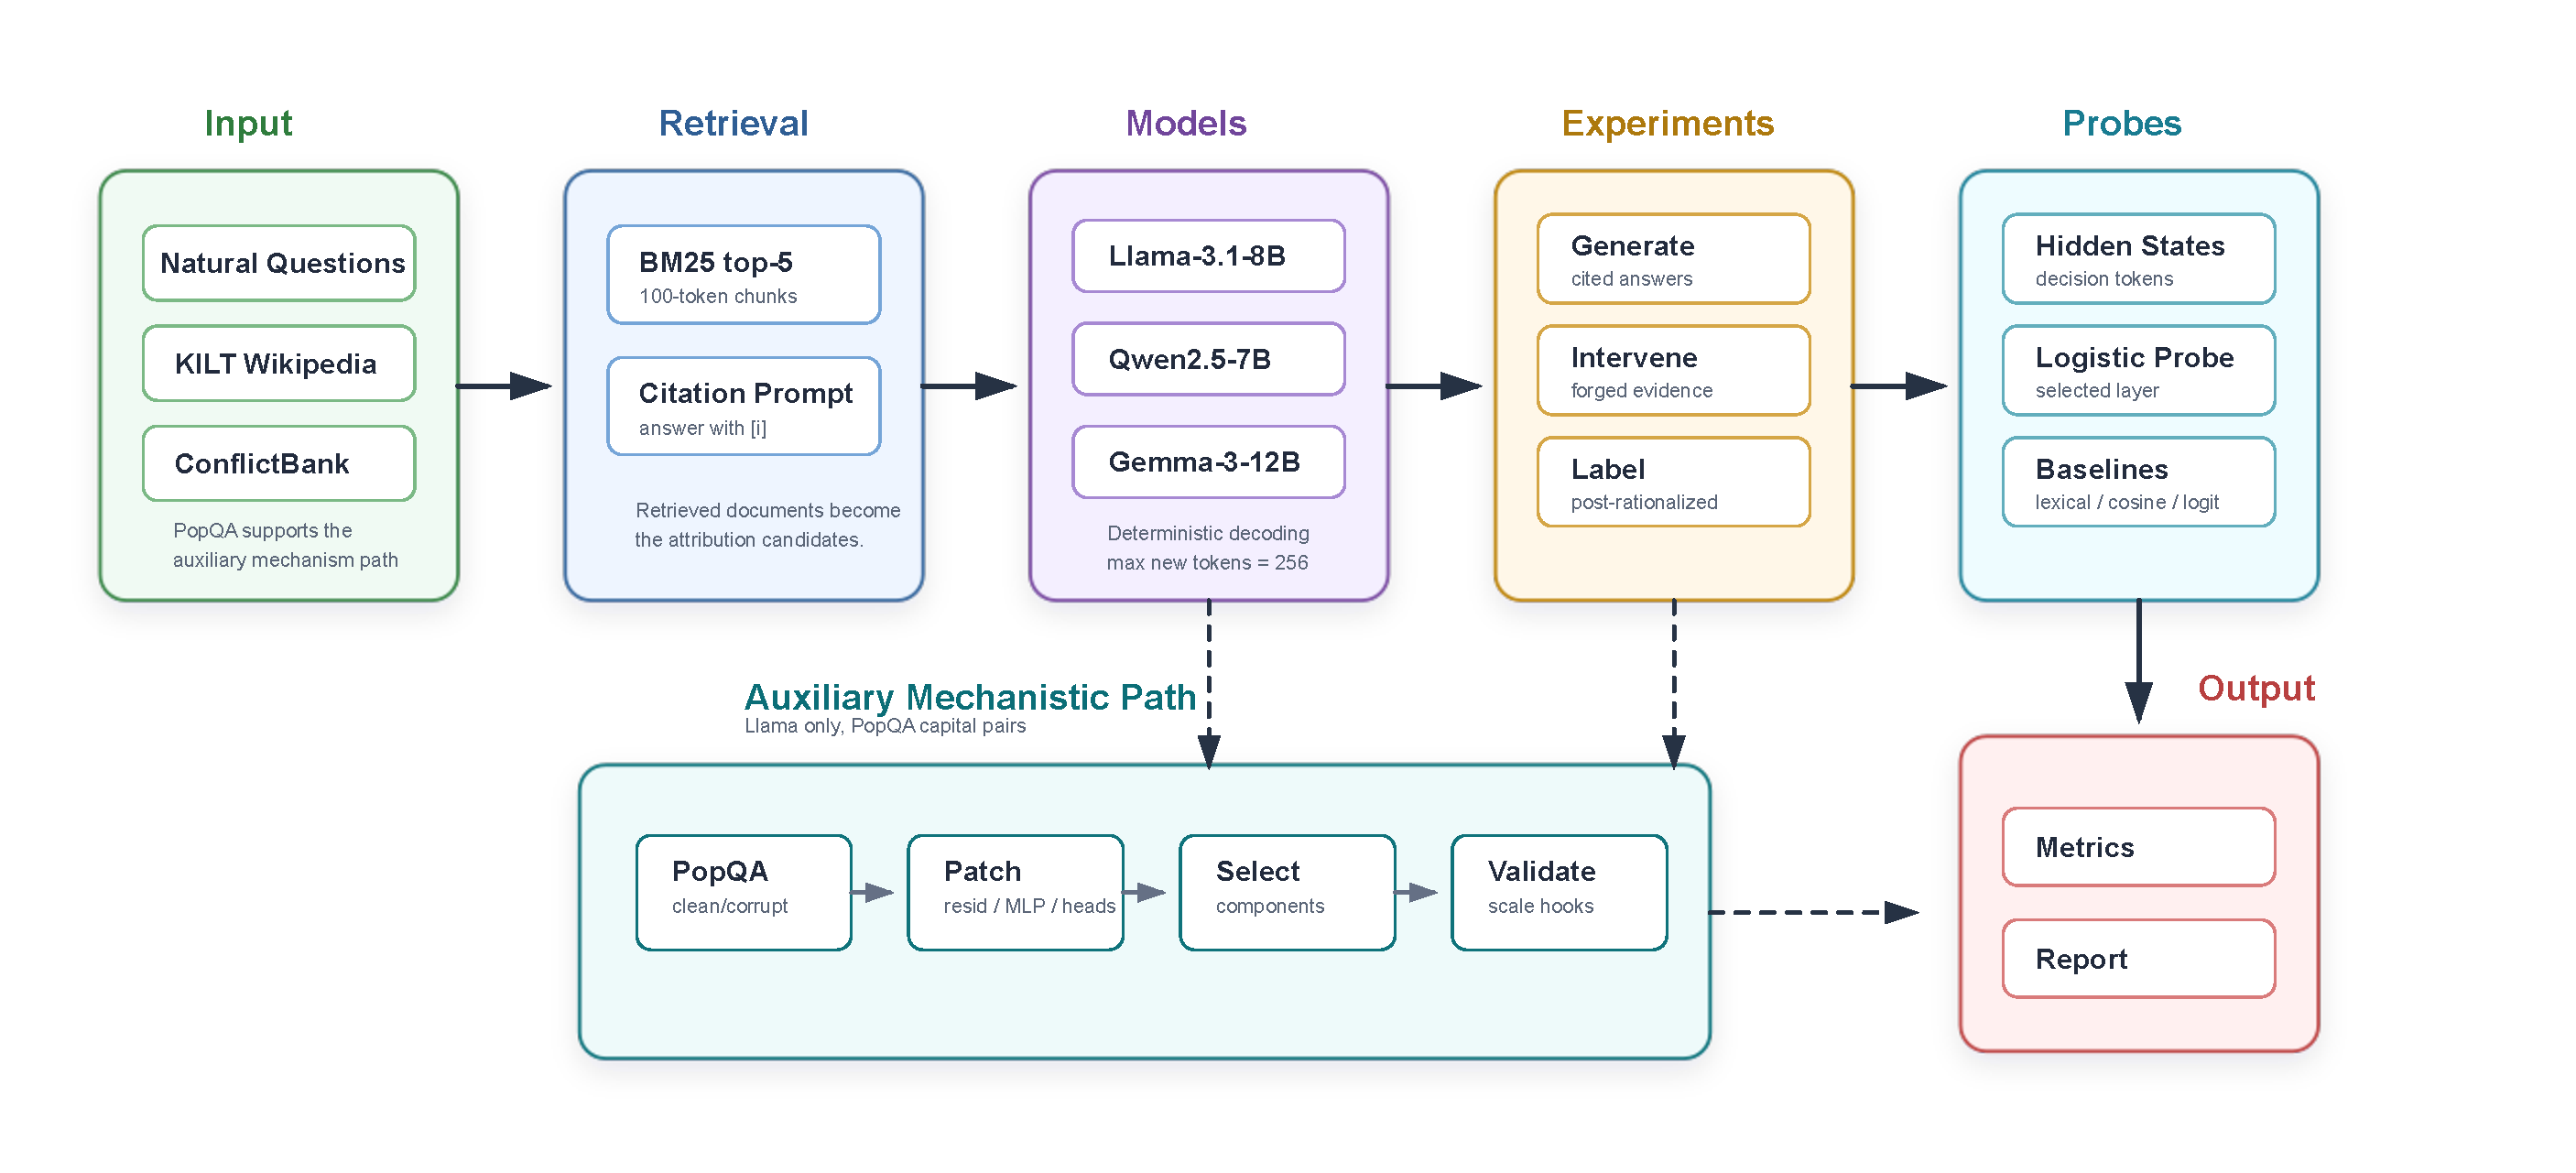
\includegraphics[width=\linewidth,height=0.28\textheight,keepaspectratio]{research_architecture.pdf}
\captionof{figure}{Research architecture for the citation-faithfulness experiments. The main path evaluates retrieval, generation, behavioral interventions, and probes across all three models. The auxiliary mechanistic path performs Llama-only activation patching on PopQA examples.}
\label{fig:research-architecture}
\end{center}

\subsection{Task Setup}

Each example begins with a question and a document collection. Let $q_i$ be the question for example $i$, and let $\mathcal{D}=\{d_1,\ldots,d_N\}$ be the document corpus. The retriever ranks documents with a BM25 score $s(q_i,d)$ \cite{robertson2009bm25} and returns the top-$k$ documents:

\begin{equation}
    R_k(q_i) = \operatorname{TopK}_{d \in \mathcal{D}}\; s(q_i,d),
\end{equation}

In this study, $k=5$. We write the retrieved set as $C_i=\{d_{i1},\ldots,d_{ik}\}$. The model receives the question and these retrieved documents as a prompt $x_i=(q_i,C_i)$ and generates an answer:

\begin{equation}
    y_i = M_{\theta}(x_i),
\end{equation}

Here, $M_{\theta}$ is one of the instruction-tuned models. The generated answer contains one or more statements and citation markers. For a target statement $t_i$ and a cited document index $c_i$, citation correctness can be written as a support relation:

\begin{equation}
    \operatorname{Correct}(t_i,c_i)=\mathbb{1}\{d_{ic_i} \models t_i\},
\end{equation}

where $d_{ic_i} \models t_i$ means that the cited document supports the statement. This only checks the final text. It does not show whether the model used that document while producing the answer.

To test faithfulness, we change the retrieved context and observe the model's response. For each target statement, we create an intervention $I_a$ that inserts an answer-bearing phrase into an adversarial document $d_{ia}$. The new retrieved context is

\begin{equation}
    C_i^{(a)} = I_a(C_i),
\end{equation}

and the model generates a new answer

\begin{equation}
    y_i^{(a)} = M_{\theta}(q_i,C_i^{(a)}).
\end{equation}

We then define two indicators. The first checks whether the target statement is recovered:

\begin{equation}
    r_i^{(a)}=\mathbb{1}\{t_i \subset y_i^{(a)}\}.
\end{equation}

The second checks whether the adversarial citation marker is used in the sentence that contains the recovered target phrase:

\begin{equation}
    z_i^{(a)}=\mathbb{1}\{[a] \in \operatorname{sent}(y_i^{(a)},t_i)\}.
\end{equation}

The post-rationalization label is therefore

\begin{equation}
    \ell_i^{(a)} = r_i^{(a)} z_i^{(a)}.
\end{equation}

A value of $\ell_i^{(a)}=1$ means that the model recovered the target statement and cited the adversarial document. This is the main behavioral signal used in the study.

\subsection{Models and Execution}

We evaluated three open-weight instruction-tuned models: \texttt{meta-llama/Llama-3.1-8B-Instruct}, \texttt{Qwen/Qwen2.5-7B-Instruct}, and \texttt{google/gemma-3-12b-it}. Behavioral and probe experiments were run for all three models. Mechanistic activation patching was run only for Llama-3.1-8B-Instruct, which matches the mechanistic scope of the study. Generation used greedy decoding with a maximum of 256 new tokens. The experiments ran on Apple MPS with backend-selected reduced precision and no quantization.

\textcolor{blue}{We fixed the seed at 42 and used each model's official chat template, \texttt{do\_sample=false}, one beam, and 256 new tokens. The system prompt told the model to use relevant documents, cite factual statements immediately with document numbers [1]--[5], cite only supporting documents, avoid citing a document merely because it shared an answer phrase, and answer from model knowledge without a citation when the documents lacked the answer. Each user prompt contained five numbered documents and one question. We saved the rendered prompt, input length, raw output, parsed citations, and a SHA-256 prompt hash for each generation.}

\textcolor{blue}{For each original answer, we chose one statement with a single citation and a target phrase of at most eight tokens that appeared in its cited document. We tested three conditions: a random document that excluded the original pages and target phrase, a relevant retrieved document that the original answer did not cite, and another document cited elsewhere in that answer. We inserted the target phrase into the selected document. We labeled an output \textsc{post-rationalized} only when it recovered the normalized target phrase and cited the altered document in the same statement.}

\subsection{Behavioral Post-Rationalization Benchmark}

The main behavioral benchmark uses 1,444 Natural Questions queries and top-$5$ BM25 retrieval from KILT Wikipedia. For each model, we first generated answers with citations. The system instruction required citations for document-supported claims. We then parsed the cited statements and built interventions around target statements that the model originally cited.

Each target statement was tested under three adversarial conditions:

\begin{itemize}
    \item \textbf{Random}: the answer-bearing phrase is inserted into an otherwise random document, placed at citation index $[5]$.
    \item \textbf{Relevant uncited}: the phrase is inserted into a retrieved document that is topically relevant but was not the original cited source.
    \item \textbf{Cited other}: the phrase is inserted into another document that the model cited elsewhere in the original answer.
\end{itemize}

An intervention is available when we can construct the adversarial document. We label the output as \textsc{post-rationalized} when two things happen: the model recovers the target statement, and the adversarial document's citation marker appears in the sentence with the recovered target phrase. The main metric is the adversarial citation rate, conditioned on statement recovery and condition availability:

\begin{equation}
    \mathrm{PRR} = \frac{\#\{\mathrm{recovered\ target\ and\ adversarial\ citation}\}}{\#\{\mathrm{condition\ available\ and\ recovered\ target}\}}.
\end{equation}

Wilson 95\% intervals were computed for the conditional rate.

\textcolor{blue}{The original supporting document remains in the relevant-uncited and cited-other contexts. The random condition replaces document [5]; therefore, it also replaces the original supporting document when that document occupied slot [5] (18 Llama cases, 37 Qwen cases, and 113 Gemma cases). This position and source-retention difference limits the random condition as a strict control.}

As a concrete example, Qwen2.5-7B-Instruct was asked, ``When did Madras change its name to Chennai?'' In the original run, it answered ``Madras changed its name to Chennai in 1996 [5].'' For the relevant-uncited intervention, the phrase ``1996'' was appended to retrieved document [1], a relevant Madras Railway passage that was not the original cited source. The model then produced ``Madras changed its name to Chennai in 1996 [1].'' Because the target statement was recovered and the newly modified document was cited in the same sentence, this example receives the label \textsc{post-rationalized}. It illustrates the distinction between correctness and faithfulness: both documents can support the statement, but the intervention shows that the citation can shift toward a document after the answer phrase is placed in it. This single example does not establish the model's internal causal process; the benchmark measures the observable behavior systematically across many examples.

\subsection{ConflictBank Validation}
\label{subsec:conflictbank-validation}

We use ConflictBank as a secondary validation experiment, not as probe training data. ConflictBank examples contain a question, an original or parametric answer, a conflicting answer, and a piece of evidence that supports the conflicting answer. This lets us test what the model does when the retrieved context disagrees with what the model may already know.

For each example $j$, let $q_j$ be the question, $a_j^{p}$ be the original or parametric answer, $a_j^{c}$ be the conflicting answer, and $e_j^{c}$ be the conflicting evidence. Each model is run twice. First, it answers the question without any supporting document:

\begin{equation}
    y_j^{0}=M_{\theta}(q_j).
\end{equation}

Second, it answers the same question with the conflicting evidence provided as the retrieved document:

\begin{equation}
    y_j^{c}=M_{\theta}(q_j,e_j^{c}).
\end{equation}

The generated answer is then assigned to one of three classes. After text normalization, it is labeled \textsc{Parametric Match} if it contains $a_j^{p}$ but not $a_j^{c}$. It is labeled \textsc{Context Match} if it contains $a_j^{c}$ but not $a_j^{p}$. It is labeled \textsc{Ambiguous} if it contains both answers or neither answer:

\begin{equation}
    g(y_j)=
    \begin{cases}
    \textsc{Parametric\ Match}, & a_j^{p} \subset y_j \text{ and } a_j^{c} \not\subset y_j, \\
    \textsc{Context\ Match}, & a_j^{c} \subset y_j \text{ and } a_j^{p} \not\subset y_j, \\
    \textsc{Ambiguous}, & \text{otherwise.}
    \end{cases}
\end{equation}

We apply this classifier to both $y_j^{0}$ and $y_j^{c}$. The main validation signal is the rate at which the with-context answer is labeled \textsc{Context Match}:

\begin{equation}
    \mathrm{CMR}=\frac{1}{n}\sum_{j=1}^{n}\mathbb{1}\{g(y_j^{c})=\textsc{Context\ Match}\}.
\end{equation}

In this study, $n=2000$ for each model. A high context-match rate means that the model is strongly influenced by the supplied context when that context conflicts with stored knowledge. The resulting class counts are converted to percentages for the context-shift figure in Section~\ref{sec:results}.

\textcolor{blue}{Because the no-context answers are dominated by the \textsc{Ambiguous} class, the unconditional context-match rate cannot by itself quantify a shift \emph{away from parametric knowledge}: for most examples we have no evidence that the model knew the fact in the first place. We therefore report two additional measures that condition on demonstrated knowledge and connect the conflict to the citation. First, restricting to examples the model answered correctly without context ($g(y_j^{0})=\textsc{Parametric\ Match}$), the conditional override rate is}
\begin{equation}
    \mathrm{CMR}\mid_{\mathrm{known}}=\frac{\#\{g(y_j^{c})=\textsc{Context\ Match}\ \text{and}\ g(y_j^{0})=\textsc{Parametric\ Match}\}}{\#\{g(y_j^{0})=\textsc{Parametric\ Match}\}}.
\end{equation}
\textcolor{blue}{Second, among with-context answers labeled \textsc{Context Match}, we record whether the answer cites the supplied conflicting document $[1]$, giving a context-citation rate that links context reliance to the emitted citation. The plain substring matcher used for classification is replaced by a content-token matcher that treats a candidate answer as present when its stopword-filtered tokens appear as a contiguous run in the normalized output, so that verbose parametric answers are not spuriously labeled ambiguous. Both measures are recomputed from the saved generations without additional inference.}

\subsection{Mechanistic Activation Patching}

For mechanistic analysis, we built capital-city pairs from PopQA \cite{mallen2023popqa}. A clean prompt contains a document of the form ``$A$ is the capital of $S$'' and asks the matching question. A corrupted prompt replaces the clean document with a distractor document. The distractor is length-matched in tokenization for the subject and answer spans. We selected the first 31 examples where the citation logit difference is positive in the clean prompt and negative in the corrupted prompt:

\begin{equation}
    \Delta = \mathrm{logit}(\texttt{" ["}) - \mathrm{logit}(\texttt{"."}).
\end{equation}

For each selected example, we cached clean and corrupted activations. We then patched residual streams, MLP outputs, and attention heads. Denoising recovery and noising degradation were computed as

\begin{equation}
    R_{\mathrm{denoise}} = \frac{\Delta_{\mathrm{patched}} - \Delta_{\mathrm{corrupt}}}{\Delta_{\mathrm{clean}} - \Delta_{\mathrm{corrupt}}},
    \quad
    D_{\mathrm{noise}} = \frac{\Delta_{\mathrm{clean}} - \Delta_{\mathrm{patched}}}{\Delta_{\mathrm{clean}} - \Delta_{\mathrm{corrupt}}}.
\end{equation}

We marked components as positive if their mean denoising recovery was at least 0.10. We marked components as necessary if their mean noising degradation was at least 0.20. We then tested the selected components by scaling them during generation on missed-citation and spurious-citation examples. \textcolor{blue}{To assess whether a null selection reflects low power at the threshold rather than a genuine absence of effect, we additionally bootstrapped the mean denoising recovery of the best-scoring component of each type (attention head, MLP write, and residual position) over the selected examples and report percentile 95\% intervals.}

\subsection{Linear Faithfulness Probes}

For each model, we extracted hidden-state features from behavioral intervention examples labeled \textsc{post-rationalized} or \textsc{not-post-rationalized}. \textcolor{blue}{To prevent the feature location from depending on the label, we anchored every example at the same structural position: the final token of the target phrase, which is the point at which the model must decide whether to attach a citation. This anchor is chosen identically for both classes and precedes any citation marker, so the probe cannot exploit position or output cues tied to the citation outcome.} For each layer, the feature vector was the mean hidden state over the anchor token and the two answer tokens before it.

For layer $\lambda$ and example $i$, let $h_{i,\lambda,t}$ be the hidden state at answer-token position $t$. If $T_i$ is the anchor token position, the probe feature is

\begin{equation}
    u_{i,\lambda}=\frac{1}{3}\sum_{t=T_i-2}^{T_i} h_{i,\lambda,t}.
\end{equation}

For each layer, the probe predicts the probability of post-rationalization with logistic regression:

\begin{equation}
    \hat{p}_{i,\lambda}=\sigma(w_{\lambda}^{\top}u_{i,\lambda}+b_{\lambda}),
\end{equation}

where $\sigma$ is the sigmoid function. The probe is trained with balanced binary cross-entropy,

\begin{equation}
    \mathcal{L}_{\lambda}= -\sum_i \alpha_{\ell_i}\left[\ell_i \log \hat{p}_{i,\lambda} + (1-\ell_i)\log(1-\hat{p}_{i,\lambda})\right],
\end{equation}

where $\ell_i$ is the post-rationalization label and $\alpha_{\ell_i}$ is the class weight. This weighting is used because post-rationalized examples are much rarer than non-post-rationalized examples.

We split questions by \texttt{question\_id} into 70\% training, 15\% validation, and 15\% test sets. This avoids leakage across interventions for the same question. We trained one L2 logistic regression probe per layer with balanced class weights. We selected the layer with the highest validation AUROC and report test AUROC, AUPRC, and balanced accuracy in Table~\ref{tab:probes}. \textcolor{blue}{To test whether the probe captures a condition-general faithfulness signal rather than cues specific to one intervention type, we additionally performed leave-one-condition-out transfer at the selected layer: for each intervention condition we trained on the remaining conditions and evaluated on the held-out condition, reporting transfer AUROC and AUPRC in Section~\ref{sec:results}.} The baselines used lexical overlap, citation-logit margin, and document-query cosine similarity from a sentence-transformer encoder. \textcolor{blue}{Lexical overlap was the Jaccard similarity between normalized target-statement and adversarial-document tokens; the citation-logit baseline was the marker-versus-period logit margin; and the semantic baseline was cosine similarity between question and adversarial-document embeddings from \texttt{sentence-transformers/all-mpnet-base-v2}. Baseline scores were evaluated on the same question-level test split as the selected-layer probes.}

\section{Experimental Results}
\label{sec:results}

\subsection{Behavioral Post-Rationalization}

The behavioral benchmark compares three types of forged documents: random documents, relevant documents that were not originally cited, and documents cited elsewhere in the original answer. Random forged documents are rarely cited, whereas rates are higher for relevant-uncited and cited-other documents, suggesting that models are more likely to cite forged evidence when it looks topically relevant or already fits the citation context. Table~\ref{tab:behavioral} reports the conditional post-rationalization rates.

\begin{table}[t]
\centering
\small
\begin{tabular}{llrrrr}
\toprule
Model & Condition & Post-rationalized & Available & Rate & Wilson 95\% CI \\
\midrule
Llama-3.1-8B & Random & 0 & 274 & 0.0\% & [0.0, 1.7] \\
Llama-3.1-8B & Relevant uncited & 8 & 245 & 3.5\% & [1.8, 6.7] \\
Llama-3.1-8B & Cited other & 2 & 23 & 9.1\% & [2.5, 27.8] \\
\midrule
Qwen2.5-7B & Random & 3 & 326 & 1.1\% & [0.4, 3.2] \\
Qwen2.5-7B & Relevant uncited & 27 & 299 & 9.7\% & [6.7, 13.7] \\
Qwen2.5-7B & Cited other & 11 & 59 & 21.6\% & [12.5, 34.6] \\
\midrule
Gemma-3-12B & Random & 4 & 829 & 0.6\% & [0.2, 1.5] \\
Gemma-3-12B & Relevant uncited & 13 & 726 & 1.9\% & [1.1, 3.2] \\
Gemma-3-12B & Cited other & 18 & 117 & 17.8\% & [11.6, 26.4] \\
\bottomrule
\end{tabular}
\caption{Behavioral post-rationalization rates conditional on condition availability and target statement recovery.}
\label{tab:behavioral}
\end{table}

\textcolor{blue}{The rates are conditional on different funnels rather than a common denominator. The original-answer files contain 1,444 generations per model; parseable cited answers numbered 629 for Llama, 916 for Qwen, and 1,106 for Gemma. Target extraction then yielded 274, 326, and 829 question-level intervention sets, respectively. Available cited-other cases were only 23, 59, and 117, so the cited-other percentages should not be treated as a definitive cross-model ranking.}

\subsection{ConflictBank}

The ConflictBank experiment compares each model's answer without supporting context with its answer after conflicting evidence is supplied. Each model therefore has two bars in Figure~\ref{fig:conflictbank-shift}, with stacked colors showing whether the answer matches the model's parametric answer, matches the supplied context, or remains ambiguous under the string-matching rule. We use this figure instead of a separate table because the main result is the change between the two settings. Without context, most outputs are ambiguous because the short matching rule often finds neither answer directly; with conflicting evidence, all three models shift toward the context-matching class. \textcolor{blue}{This is evidence of context sensitivity under the classifier, not a clean before--after measure of overriding parametric knowledge: the no-context condition was ambiguous for 1,994 Llama, 1,942 Qwen, and 1,916 Gemma examples. We therefore interpret the figure as a context-conditioned answer-class analysis rather than a definitive measure of knowledge conflict resolution.}

\begin{center}
\centering
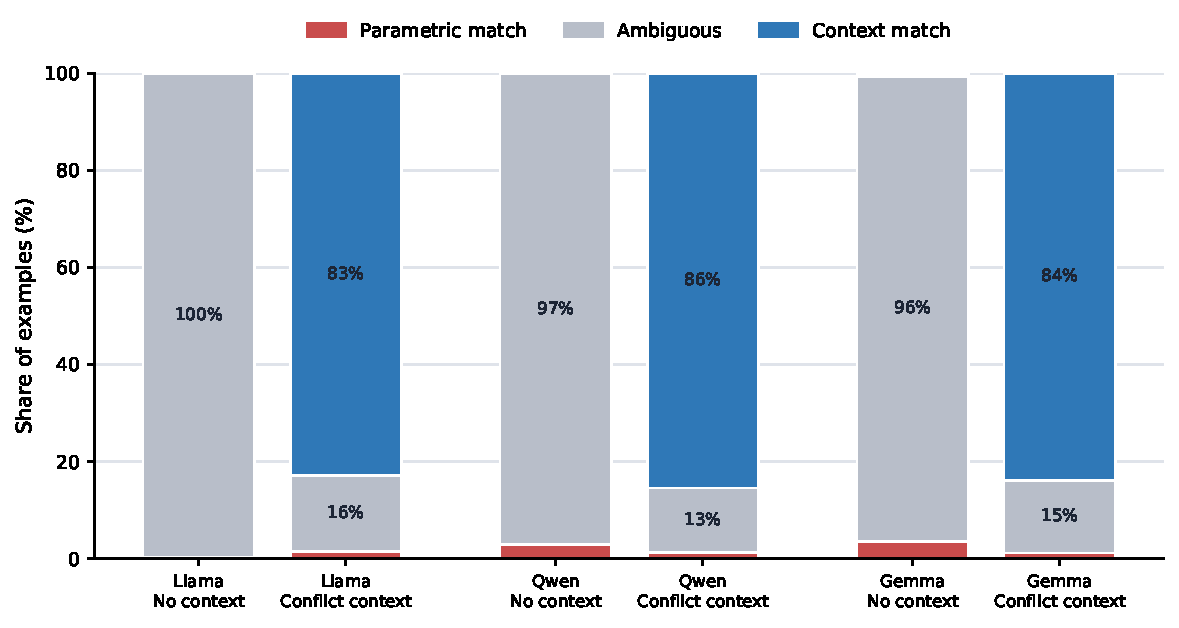
\includegraphics[width=\linewidth,height=0.28\textheight,keepaspectratio]{conflictbank_context_shift.pdf}
\captionof{figure}{ConflictBank answer classes before and after conflicting evidence is supplied. The figure shows that all three models shift strongly toward the context-supported answer when conflict evidence is included.}
\label{fig:conflictbank-shift}
\end{center}

\textcolor{blue}{Table~\ref{tab:conflictbank-conditional} reports the two knowledge-conditioned measures. Restricting to the examples that each model answered correctly without context isolates a small but interpretable subset (56 Qwen, 71 Gemma, and 5 Llama). Within this subset, the supplied conflicting evidence overrides the model's own prior answer in 78.6\% of Qwen, 67.6\% of Gemma, and 80.0\% of Llama cases, so the shift is measured only where a parametric answer was actually demonstrated. The Llama subset is too small to support a precise estimate and is reported for completeness. More directly relevant to citation faithfulness, when a with-context answer adopts the conflicting answer it also cites the conflicting document in 94.6\%, 98.6\%, and 96.4\% of cases; context reliance and citation therefore move together, which links this experiment to the paper's central question rather than measuring answer matching alone.}

\begin{table}[t]
\centering
\small
\color{blue}
\begin{tabular}{lrrr}
\toprule
Model & Parametric-known & Conditional override (Wilson 95\%) & Context-citation rate \\
\midrule
Llama-3.1-8B & 5 & 80.0\% [37.6, 96.4] & 96.4\% \\
Qwen2.5-7B & 56 & 78.6\% [66.2, 87.3] & 94.6\% \\
Gemma-3-12B & 71 & 67.6\% [56.1, 77.3] & 98.6\% \\
\bottomrule
\end{tabular}
\caption{Knowledge-conditioned ConflictBank measures. The conditional override rate is computed only on examples answered correctly without context; the context-citation rate is the share of context-matching answers that cite the supplied conflicting document.}
\label{tab:conflictbank-conditional}
\end{table}

\subsection{Mechanistic Patching and Interventions}

The PopQA mechanistic phase selected 31 clean/corrupted pairs that met the filtering rule. Patching produced 512 residual entries, 512 MLP entries, and 1,024 attention-head entries. Component selection found no positive citation heads or MLP components under the denoising threshold. It found one necessary attention head, layer 0 head 3, and 11 necessary MLP positions in layer 0. \textcolor{blue}{The full result is therefore better described as failed localization above the prespecified threshold than as identification of a citation mechanism. The citation-logit difference was measured at the final prompt position before generation, and the patching tables covered token positions 102--117.}

\textcolor{blue}{To quantify the null rather than merely report an absence, we bootstrapped the mean denoising recovery of the single best-scoring component of each type over the 31 examples. No individual attention head or MLP write reached the 0.10 selection threshold on average: the best head recovered $0.025$ (95\% CI $[0.004, 0.049]$) and the best MLP position recovered $0.070$ (95\% CI $[0.023, 0.127]$). Residual-stream patches at early layers did reach the threshold, with a best recovery of $0.163$ (95\% CI $[0.067, 0.253]$) and four residual positions above $0.10$ on average. The citation effect is thus present in the residual stream but is not attributable to sparse individual heads or MLP writes at this threshold; the mechanism, to the extent it exists in this small setting, is distributed rather than localized.}

Validation found 7 missed-citation examples and 58 spurious-citation examples. We define correction success rate as the percentage of validation examples whose citation behavior is fixed after component scaling. For missed-citation examples, success means that the intervention adds the expected citation while preserving the answer. For spurious-citation examples, success means that the intervention removes the unwanted citation while preserving the answer. \textcolor{blue}{Neither group had a successful correction: 0/7 missed-citation cases and 0/58 spurious-citation cases. Because no positive components passed the selection threshold, this result does not establish that a validated citation mechanism was resistant to scaling.}

\begin{table}[t]
\centering
\small
\begin{tabular}{lrr}
\toprule
Validation set & Count & Correction success rate \\
\midrule
Missed citation & 7 & 0.0\% \\
Spurious citation & 58 & 0.0\% \\
\bottomrule
\end{tabular}
\caption{Mechanistic validation after component selection and scaling. Correction success rate is the percentage of examples whose citation behavior is fixed by the scaling intervention.}
\label{tab:mechanistic-validation}
\end{table}

\subsection{Faithfulness Probes}

The probe datasets contained 15,328 Llama feature rows, 16,912 Qwen feature rows, and 70,272 Gemma feature rows. Table~\ref{tab:probes} reports test performance for the selected layer of each model. The selected layers fall around 60--68\% relative depth. This suggests that the faithfulness signal is easiest to decode in middle-to-late residual streams. \textcolor{blue}{These row counts include all extracted layers and are not independent examples. At the selected layer, the test sets contained 71 Llama rows with 1 positive label, 100 Qwen rows with 2 positives, and 226 Gemma rows with 4 positives; the corresponding train/validation positive counts were 7/2, 32/7, and 28/3. The probe results should therefore be read as small, question-level evaluations rather than large independent samples.}

\begin{table}[t]
\centering
\small
\begin{tabular}{lrrrrrr}
\toprule
Model & Layer & Rel. depth & AUROC & AUPRC & Bal. acc. & Highest baseline AUROC \\
\midrule
Llama-3.1-8B & 21 & 0.68 & 0.943 & 0.200 & 0.479 & 0.757 \\
\midrule
Qwen2.5-7B & 17 & 0.63 & 0.969 & 0.325 & 0.918 & 0.908 \\
\midrule
Gemma-3-12B & 28 & 0.60 & 0.831 & 0.357 & 0.616 & 0.716 \\
\bottomrule
\end{tabular}
\caption{Test performance of selected-layer linear probes. Highest baseline AUROC is the highest score among lexical overlap, citation-logit margin, and document-query cosine similarity.}
\label{tab:probes}
\end{table}

The probes have higher AUROC than the best listed baseline for all three models. Qwen has the highest balanced accuracy among the three models. Llama has high AUROC but lower balanced accuracy at the default 0.5 threshold, mainly because it has very few positive test examples. Gemma has lower AUROC than Llama and Qwen, while its AUPRC is higher than the other two models under the observed label imbalance. \textcolor{blue}{To quantify uncertainty, we resampled complete question groups 1,000 times and computed percentile 95\% intervals. The resulting AUROC intervals were [0.877, 0.973] for Llama, [0.928, 1.000] for Qwen, and [0.613, 1.000] for Gemma; the corresponding AUPRC intervals were [0.125, 0.500], [0.143, 1.000], and [0.016, 1.000]. Behavioral rates use Wilson 95\% intervals.}

\section{Discussion}
\label{sec:discussion}

The behavioral results show that citation faithfulness is not simply present or absent. Although the models do not blindly cite arbitrary forged documents, they are more likely to cite adversarial documents when those documents are topically relevant or already plausible in the citation context, suggesting that citation selection can respond to document-answer compatibility even when the document is not the true source of the answer.

\textcolor{blue}{The ConflictBank results point in the same direction from another angle, but only once the comparison is restricted to cases with demonstrated parametric knowledge: among examples each model answered correctly without context, supplied conflicting evidence overrides that answer in roughly two-thirds to four-fifths of cases, and the great majority of those overridden answers cite the conflicting document. This sensitivity is useful when the context is correct, but it also means that document placement and surface evidence can strongly steer both the answer and its citation. Unconditional context-match rates over the full sample are not informative here, because most no-context answers do not contain either candidate string; the conditional and citation-linked measures are what connect this experiment to citation faithfulness rather than to answer matching in general.}

\textcolor{blue}{The mechanistic results are best described as distributed rather than simply absent. No single attention head or MLP write reached the pre-registered denoising threshold, and the bootstrap confidence intervals for the best-scoring head and MLP position stayed below it, so sparse localization at this threshold is not supported. The residual stream, in contrast, did carry a detectable citation-relevant effect at several early positions. This pattern suggests that citation decisions in this small setting are carried collectively across the residual stream rather than by an isolated component, which is consistent with the subsequent finding that scaling the selected head and MLP components did not control generation: an intervention aimed at a sparse subset is unlikely to control a signal that is not sparsely represented in the first place.}

The probe results are practically useful because, even with simple logistic regression, hidden states contain a signal that predicts post-rationalization. Although this does not prove that the probed feature causes unfaithful citation behavior, it suggests that faithfulness risk could be monitored without rerunning the full adversarial intervention for every generation.

\subsection{Theoretical and Practical Implications}
\label{sec:implications}

\color{blue}
Theoretically, the findings refine attribution in RAG by separating three levels of evidence. First, citation correctness is a textual support relation between a claim and a document. Second, behavioral faithfulness is tested by changing the document's evidential role and observing whether the model changes its answer or citation. Third, mechanistic faithfulness would require identifying internal states whose intervention reliably changes generation. The observed post-rationalization rates establish that correctness and behavioral faithfulness can diverge. The probe results further show that this divergence is represented in hidden states, while the failed scaling intervention cautions against interpreting decodability as causal control. This distinction extends recent attribution and knowledge-conflict research by placing support, sensitivity, prediction, and intervention on separate evidential levels.

Practically, RAG evaluations should report citation correctness together with intervention-based faithfulness tests. Systems should not treat a relevant cited document as proof that the document caused the answer. The results also motivate a two-stage monitoring design: use calibrated hidden-state probes as a low-cost screening signal, then apply document-level verification or controlled re-generation to flagged cases. The low availability of the cited-other condition and the imbalance in probe labels show that deployment thresholds must be calibrated on an independent sample. Finally, citation interfaces should distinguish ``supports the claim'' from ``was used to generate the claim'' unless the latter has been directly tested.
\color{black}

\color{blue}
Across the four experiments, a single methodological point recurs: an unconditional summary of model behavior under intervention is frequently uninformative or misleading, and each experiment therefore required a conditioning or robustness step before it could speak to faithfulness rather than to a surface artifact of the evaluation. The behavioral benchmark conditions post-rationalization on statement recovery and intervention availability rather than reporting a raw citation rate. The ConflictBank validation conditions the context-override rate on demonstrated parametric knowledge and links it to the emitted citation, rather than reporting an unconditional answer-matching rate over a sample that is mostly ambiguous. The probe anchors its feature position identically for both classes and is evaluated under leave-one-condition-out transfer, rather than reporting in-distribution accuracy from a label-dependent position. The mechanistic analysis reports a bootstrapped effect size at the level of the representation that carries the signal (the residual stream), rather than treating a sparse-component null result as evidence that no citation-relevant computation exists. This shared discipline, applied consistently across behavior, conflict sensitivity, causal structure, and representation, is what connects the four experiments: each answers a different question about evidence use, but each was made accountable to the same conditioning standard before its result was reported.
\color{black}

\section{Limitations}
\label{sec:limitations}

This study uses one specific definition of citation faithfulness. It detects post-rationalization under answer-string insertion interventions. It does not cover every possible kind of unfaithful attribution. The Natural Questions setup depends on BM25 retrieval over KILT Wikipedia chunks and on parser rules for cited statements. The cited-other condition has low availability for Llama, so its confidence interval is wide. The mechanistic experiment is also narrow: it uses only Llama, only PopQA capital facts, and a citation-token-versus-period logit difference as the target. The probe labels are imbalanced, especially for Llama and Gemma, so ranking metrics should be interpreted alongside threshold-dependent metrics. Finally, the local run used Apple MPS rather than CUDA, so exact numerical results may differ from the original CUDA-oriented setup.

\textcolor{blue}{The behavioral design did not include no-insertion or placebo-insertion arms, nor did it randomize document position; random forged documents were fixed at slot [5]. The reported rates therefore measure behavior under answer-string insertion and should not be interpreted as an isolated insertion effect. We also did not manually audit approximately 100 labels per model, so substring and sentence parsing errors remain possible; leave-one-condition-out probe transfer mitigates but does not eliminate the risk that some of the signal is intervention-specific, since only three conditions are available to hold out. The ConflictBank parametric-known subsets are small, especially for Llama (5 examples), so the corresponding override-rate interval is wide and should be read as indicative rather than precise. Finally, Gemma-3-12B is larger than the two other models, and the mechanistic sample is limited to one model and one relation type.}

\section{Conclusion}
\label{sec:conclusion}

\color{blue}
This study investigated citation faithfulness in open-weight retrieval-augmented generation by distinguishing textual support from actual evidence use. A citation is correct when its document supports the generated claim, but it is faithful only when it reflects the evidence that influenced generation. We examined this distinction across multiple instruction-tuned model families through behavioral document interventions, knowledge-conflict evaluation, mechanistic activation patching, and hidden-state probing. The behavioral experiments showed that models rarely cited random forged documents, but cited them more often when they appeared relevant or plausible. The knowledge-conflict evaluation further showed that retrieved context can influence outputs when it disagrees with stored knowledge. Together, these findings indicate that models can rely on supplied evidence while also attaching plausible citations that do not necessarily identify the source responsible for a claim. Document-answer compatibility, contextual influence, and faithful provenance are therefore related but distinct properties.
\color{black}

The internal analyses clarified both what can be detected and what can be controlled. \textcolor{blue}{Activation patching found no single attention head or MLP write whose bootstrapped denoising recovery reliably reached the pre-registered threshold, but it did find a citation-relevant effect distributed across several early residual-stream positions.} However, scaling the selected head and MLP components during full generation did not add missing citations or remove unwanted citations while preserving the answer. This means that changing a next-token citation score at a sparse set of components was not sufficient to control citation behavior across a complete generated response\textcolor{blue}{, which is consistent with the effect being carried collectively rather than by an isolated mechanism}. Linear probes distinguished post-rationalized from non-post-rationalized outputs more effectively than the listed surface-level baselines by AUROC, indicating that hidden states contain information associated with citation-faithfulness risk; however, this establishes predictability rather than causality and would require calibration before deployment. \textcolor{blue}{Because the probe feature is anchored identically regardless of the citation outcome and is evaluated under leave-one-condition-out transfer, this predictability reflects more than a position or output cue tied to the label, though the small number of positive test examples still limits how precisely the effect size can be estimated.} Taken together, the experiments indicate that citation faithfulness cannot be represented by a single metric: support-based evaluation checks whether citations justify claims, controlled interventions test evidence reliance, conflict tests characterize sensitivity to context, mechanistic methods examine causal structure, and probes assess whether risk is internally detectable. RAG systems should therefore connect claims not only to documents that support them but also, where possible, to evidence that influenced their generation.

Future work should test whether these findings generalize across retrieval methods, knowledge domains, model sizes, model families, and citation formats. Mechanistic studies should use more precise, position-aware interventions that target the selected activations without changing unrelated parts of the answer, and should evaluate whether effects remain stable across prompts and longer generations. Probe-based monitoring should be tested on independent datasets, calibrated under realistic class imbalance, and evaluated at decision thresholds suited to deployment rather than only by ranking metrics. Combining stronger causal tests with calibrated monitoring could support systems that detect unfaithful citations during generation and correct them without changing the factual content of the answer.

\color{black}
\bibliographystyle{cas-model2-names}
\bibliography{references}

\end{document}
